%!TEX root = ../Main.tex

\chapter{Design}
\section{Design Patterns}
\subsection{State Machine Pattern}
The state machine pattern has been used to develop the system. This is partly done in order to structure the general flow of the algorithm, and partly in order to support concurrent development of the algorithm, as different parts of the algorithm can be implemented simultaneously as different states.

Figure \ref{fig:STM_diagram} shows the state machine diagram for system. It can be seen that the general flow of the system is as follows:
\begin{enumerate}
	\item Set up system.
	\item Create initial population.
	\item Evaluate generation.
	\item If stopping criterion is met, save population and stop. Else-  create new generation, then return to step 3.
\end{enumerate}


\begin{figure}[H]
	\centering
	{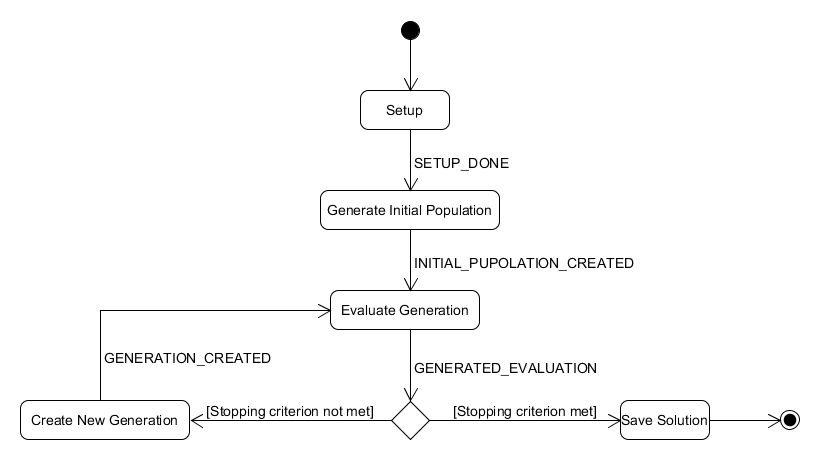
\includegraphics[width=\textwidth]{Images/STM_ROGSAnne.PNG}}\\[0.5cm]
	\caption{State machine diagram for the developed system.}
	\label{fig:STM_diagram}
\end{figure}

To get an overview of the the entire system an activity diagram has been made. This diagram illustrates how the control of the system flows and has a lot in common with the state diagram which is why a lot of the states carries over to this diagram. The activity diagram can be seen on \cref{fig:Activity_diagram}.

\begin{figure}[H]
	\centering
	{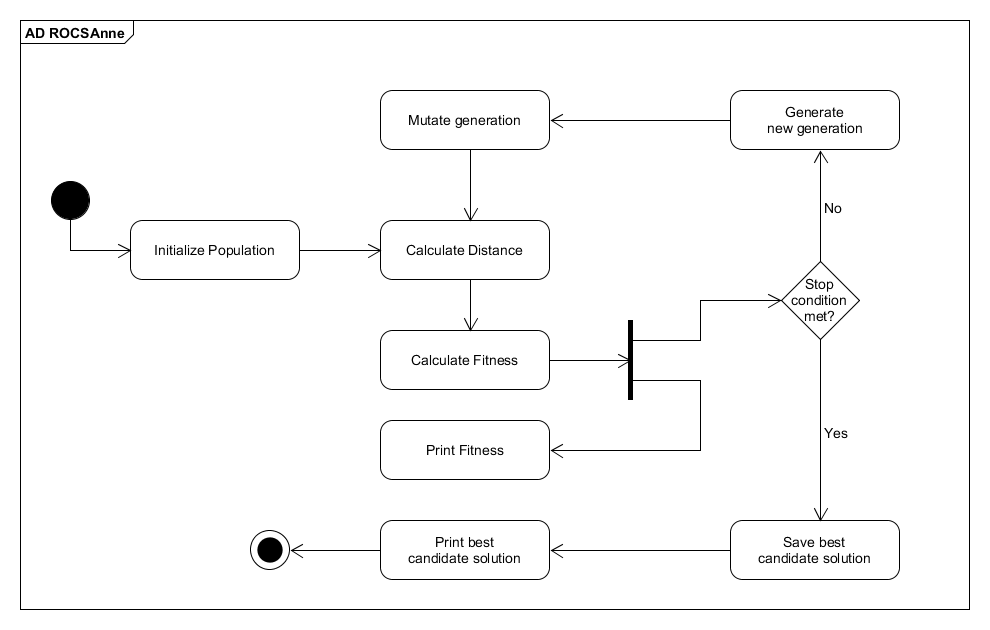
\includegraphics[width=\textwidth]{Images/AD_ROGSAnne.PNG}}\\[0.5cm]
	\caption{State machine diagram for the developed system.}
	\label{fig:Activity_diagram}
\end{figure}



\subsection{Double buffering}
The implemented algorithm operates with two buffers, one for the new generation and one for the old generation. This means when a new generation is generated the memory is allocated for the new generation beforehand. The memory for the new generation could also have been allocated dynamically which would require less memory. But, by allocating the memory beforehand makes it possible to parallelize the process of generating a new generation in the future.\\   
State pattern is the only software design pattern used in this system. 



\subsection{Command Pattern}
The command pattern will be utilized in the creation of new generations. This is done to add the possibility of parallellizing the process of creating samples in the new generation. By creating a command queue and letting different instances of the class that creates samples \textit{(creators)} execute the commands, it is possible to "order" the creation of a certain amount of new samples, and then let the execution be up to the scheduler. This way, design space exploration can be carried out, with evaluation of execution speed versus resources used.